\section{Test Beam Analysis}

With a proper e-map we can get a picture of the incident particle and observe its path and where it deposited its energy. Since the particle does not deposit all of its energy in a single scintillator tile this is critical when trying to recreate the particle energy. It is also important that there are often a variable amount of scintillator tiles in a single depth channel as shown in figure~\ref{fig:emap} which shows 4 scintillator tiles in depth 5 and 3 scintillator tiles in depth 4. Looking at the results in the plot to the left it explains why there is more energy deposited in depth 5 rather than depth 4. 

\begin{figure}
\centering
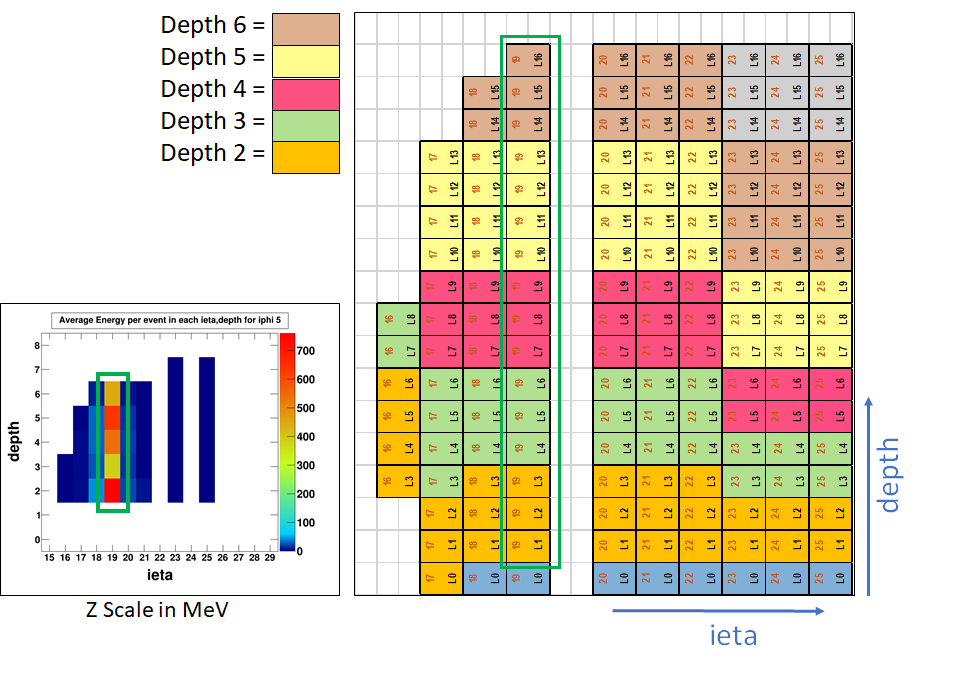
\includegraphics[width=\linewidth]{Figures/eplot.png}
\caption{This shows the relationship between the emap on the left showing which contains a geometric layout of the scintillator tiles in a single iphi slice and the data plots in a run with 150 GeV muons.}
\label{fig:emap}
\end{figure}

Muons are useful for many things but when trying to recreate the energy of the particle it is easier to use pions. The reason for this is that muons tend to go through the detector depositing a small portion of the energy but not being entirely stopped. This can be seen in figure~\ref{fig:emap} which shows the muons depositing a consistent amount of energy in each of the depths even the far ones. One the other hand figure~\ref{fig:pionmap} shows a similar plots with a pion run. This shows that the pions hit the scintillator tiles in depth 2 depositing a large portion of their energy and depositing less and less in the next depths with basically nothing in the last depth. There is also more significant spread compared to the muon run which shows the muons going straight through while the pions leave some energy in the neighboring channels.

\begin{figure}
\centering
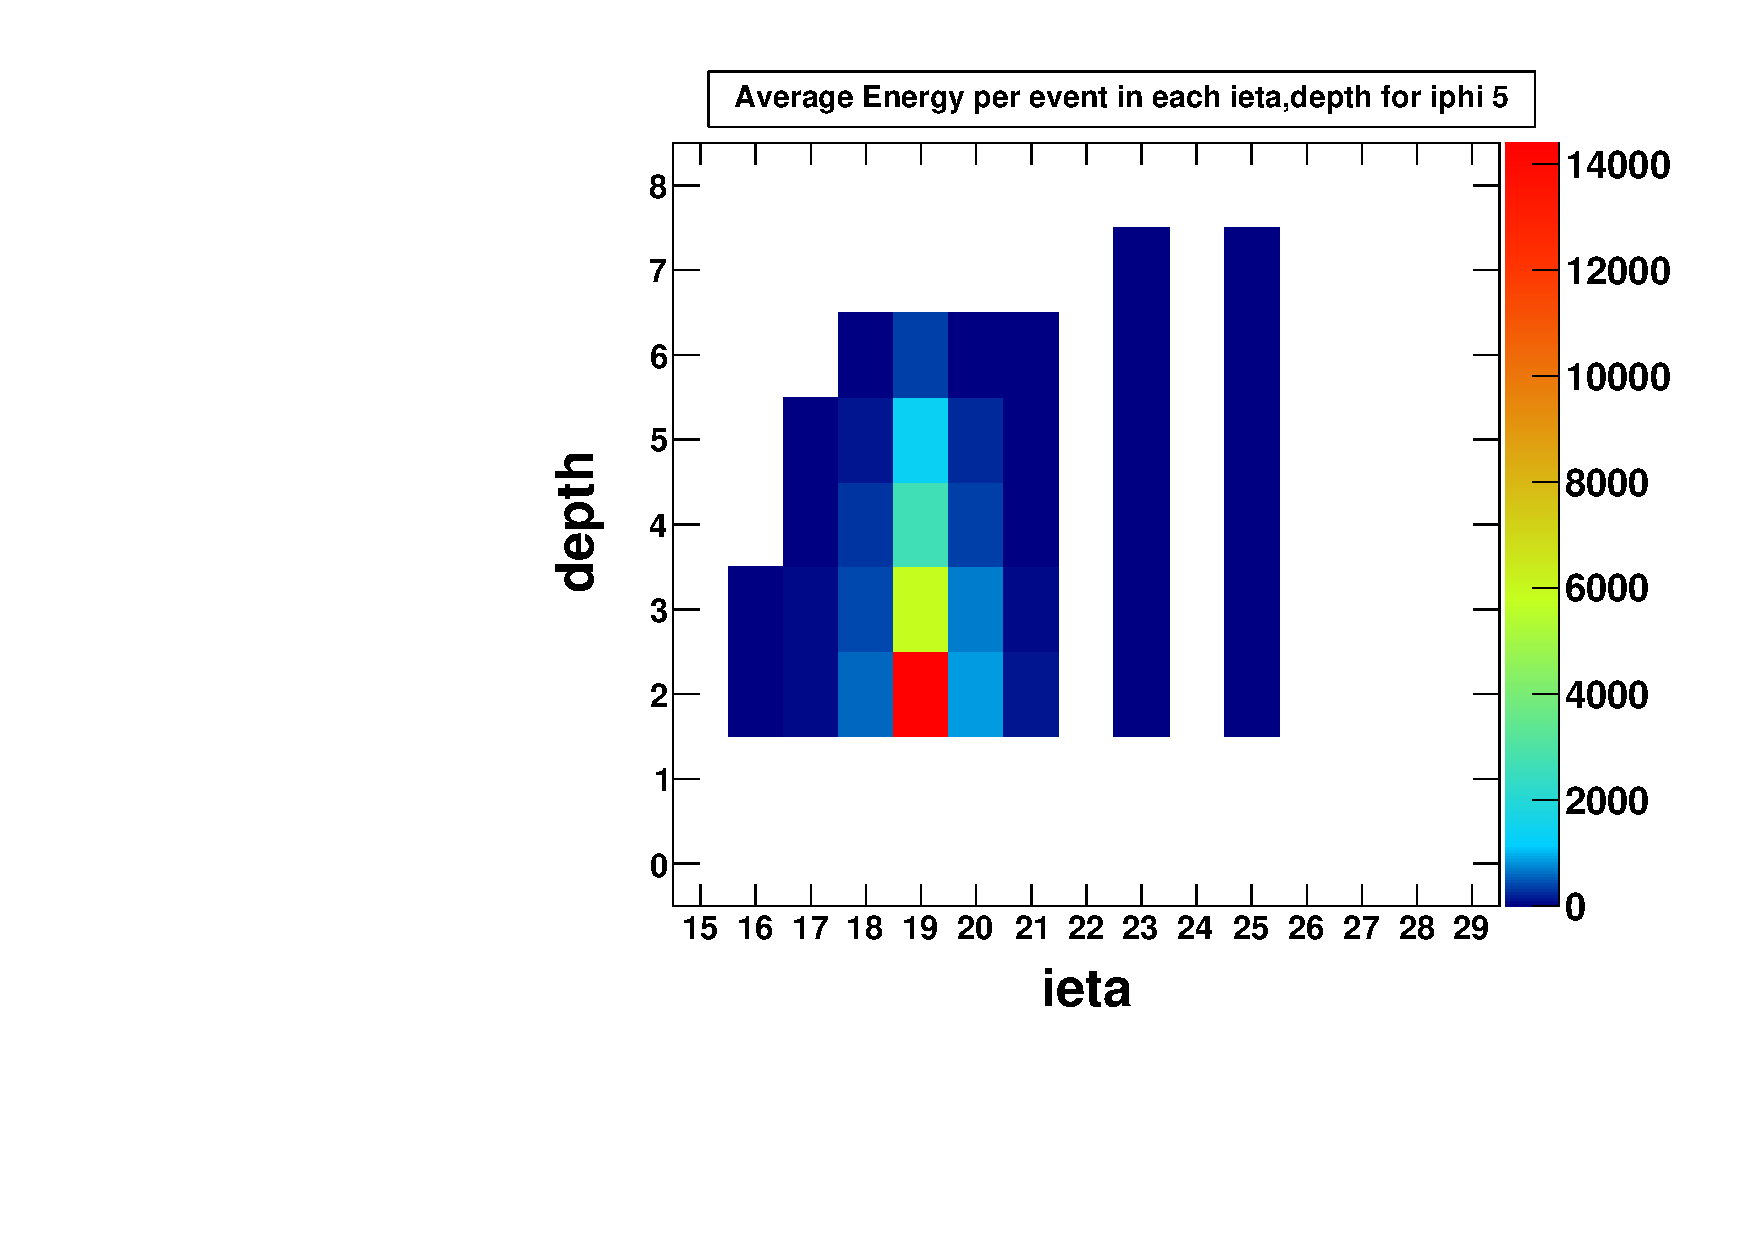
\includegraphics[width=0.7\linewidth]{Figures/pionrun.pdf}
\caption{This shows the recreation of an event with 50GeV pions showing the pions aimed at iphi 5 ieta 19 and the energy deposited in each channel z scale in MeV.}
\label{fig:pionmap}
\end{figure}

To recreate the energy of the incident particle we can look at plots such as figure~\ref{fig:pioncharge} which shows the mean output charge in a 50GeV pion run. By looking at this output charge and the output charge of the other channels we can find what portion of the particles energy was deposited in this channel and then going by the known energy of the particle how much energy was deposited to produce this output charge. 

\begin{figure}
\centering
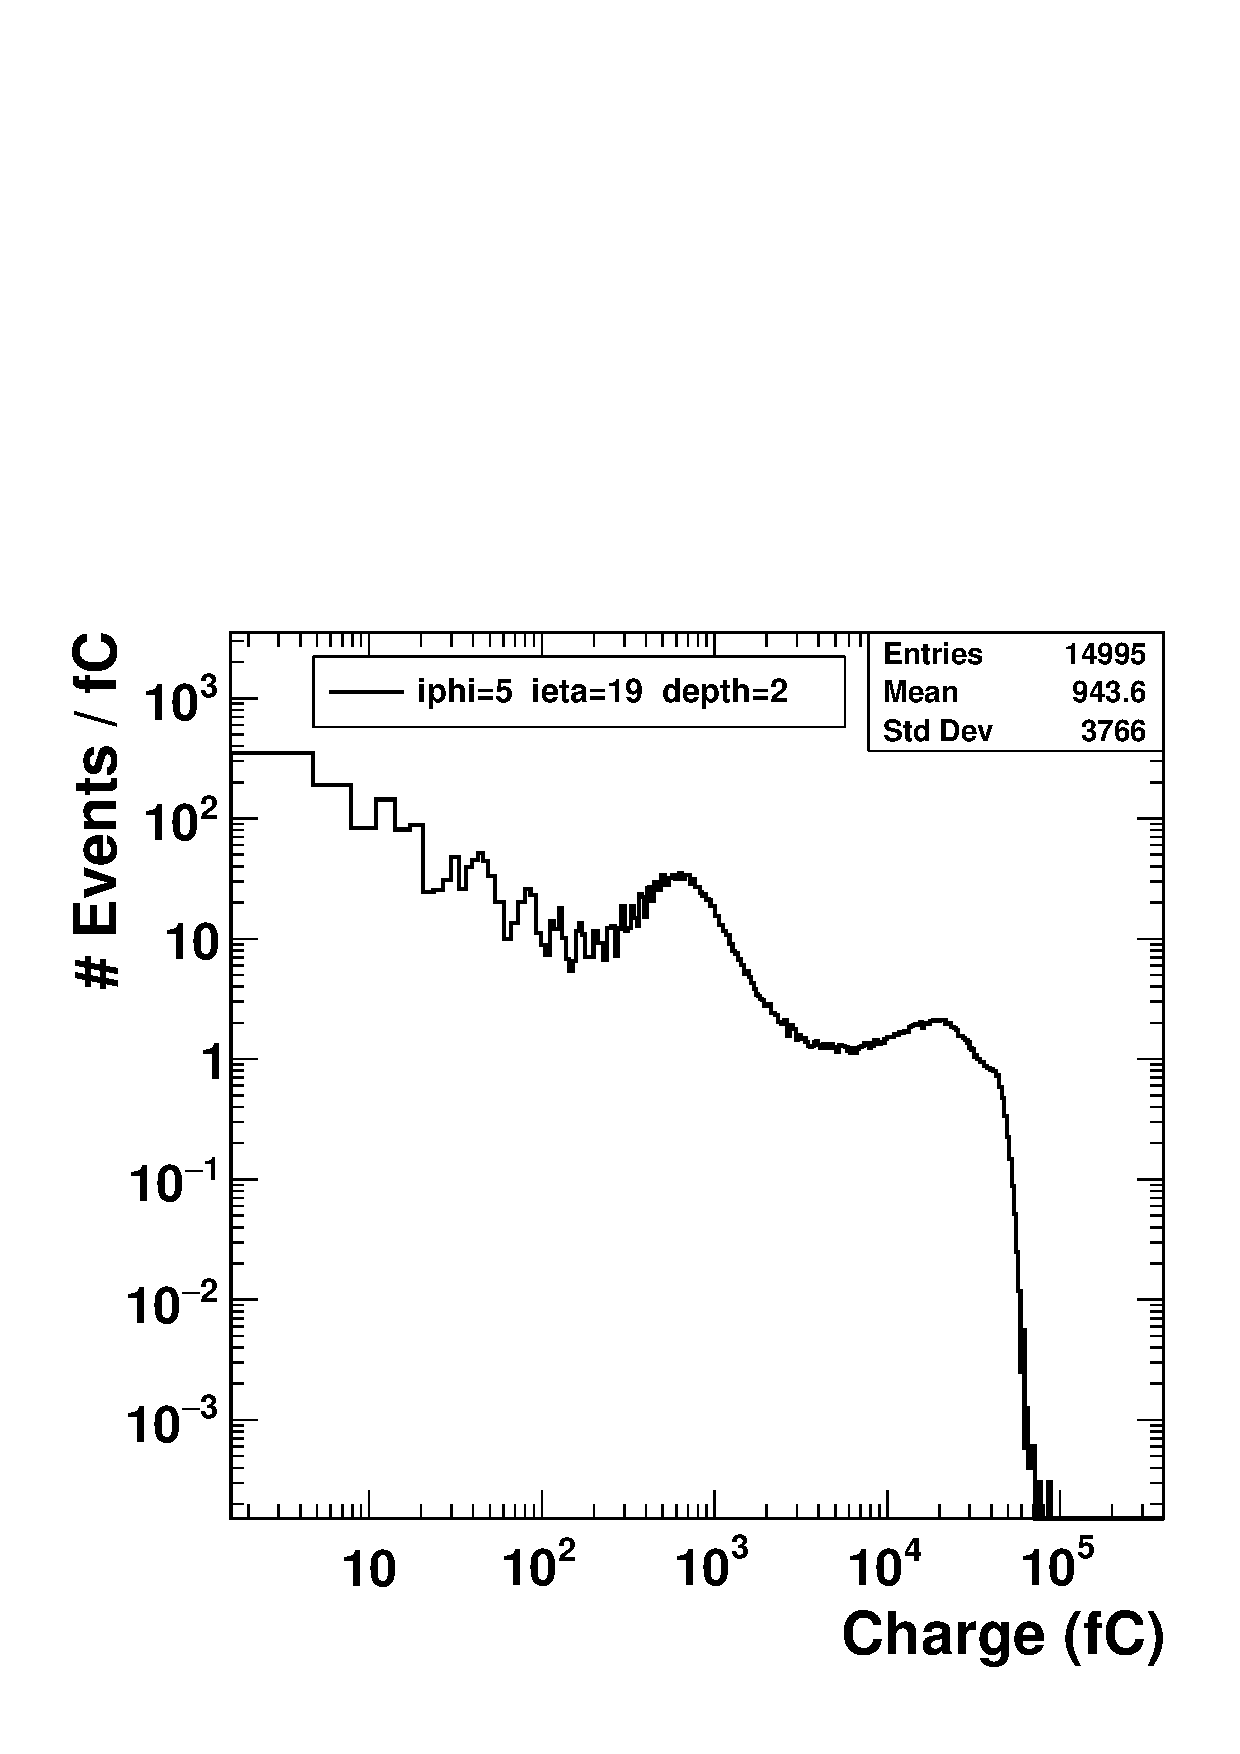
\includegraphics[width=0.7\linewidth]{Figures/pioncharge.pdf}
\caption{This shows the number of events that produces output charge in the SiPM. The peak in the middle shows the average output charge in response to the incident particles at this energy.}
\label{fig:pioncharge}
\end{figure}

One of the key things in doing a pulse shape analysis using test beam data is the timing information. In the test beam we take two different timing information. The first comes from the QIE chips in the readout modules. The readout modules measure the output charge of the SiPM over 250ns and the information is binned into 10 time samples each 25ns long. The output pulse of the SiPM is about 75ns long so it usually stays confined to 3 or 4 time samples. In addition we also take what is called a Time to Digital Converter (TDC) value. This value stores at what time in the 250ns span the output charge of the SiPM crossed a threshold with a 0.5ns resolution. Since the output charge starts out below this threshold, the TDC value should give the the start of the output pulse of the SiPM. One of the problems with the TDC value is that it could be affected by the amplitude of the output pulse as a high amplitude will cross this threshold earlier. To extract the pulse shape we can do something called a phase scan. In a phase scan we delay starting the taking of data by something less than 25ns. Since the pulse does not come in in time sample 0 we do not loose any of the pulse but simply move parts of the output pulse into different time samples. By doing this we can extract the pulse shape with a resolution much greater than 25ns. 

\begin{figure}
\centering
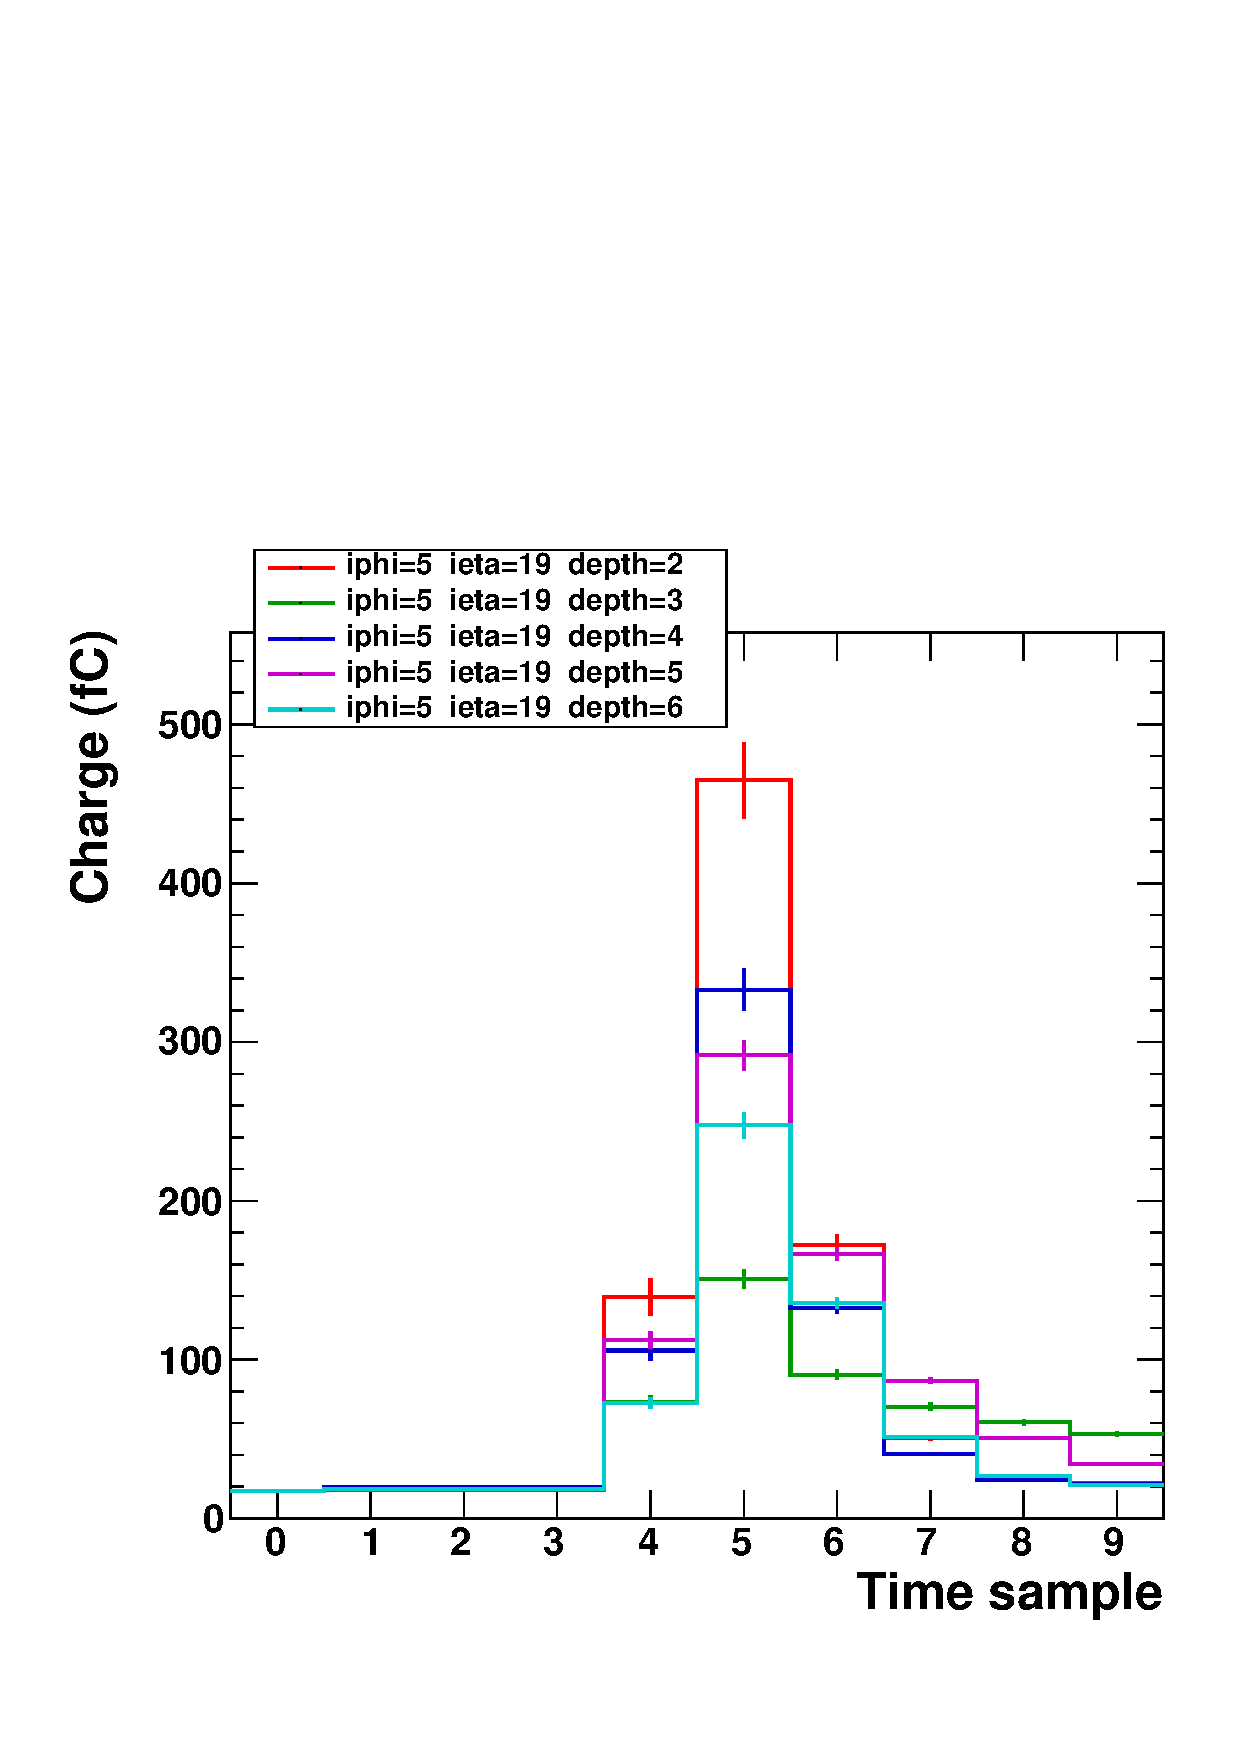
\includegraphics[width=0.7\linewidth]{Figures/Pulse.pdf}
\caption{A histogram of the output pulse of the readout modules binned in 25ns bins. This is from a run with 150GeV muons aimed at iphi5 and ieta 19. This plot shows the output pulse of the different depths at that location.}
\label{fig:PulSh}
\end{figure}

There is also the trigger information. This timing information comes from the test beam equipment that signals the back end electronics to store the data from the readout modules. 

